Based on a principal component analysis of the data (excluding the first columns including only identifier information like state names) there appear to be some potential problems with outliers.

[PCA figure with outliers and attributes removed]

We are not yet sure how best to deal with these, but in order to explore our data we also performed principal componenet analysis on our data set with some of the biggest outliers removed.

[PCA figures without outliers and attributes removed]

The above pictures illustrate our results, when we dealt with missing values by removing the corresponding attribute completely. We also performed PCA after removing data objects with missing values instead, see below

[both pictures (outliers and no outliers) of PCA with objects removed]

We also did PCA where we simply put the means along attributes instead of missing values, producing the following principal components.

[both pictures of PCA with filled means]

Investigating the work others have performed on the data, leads us to believe that considerably better preprocessing can be done to the data. As an example, we have performed principal component analysis also on the normalized data set produced by [WHO].

\begin{minipage}{0.4\textwidth}
\begin{figure}
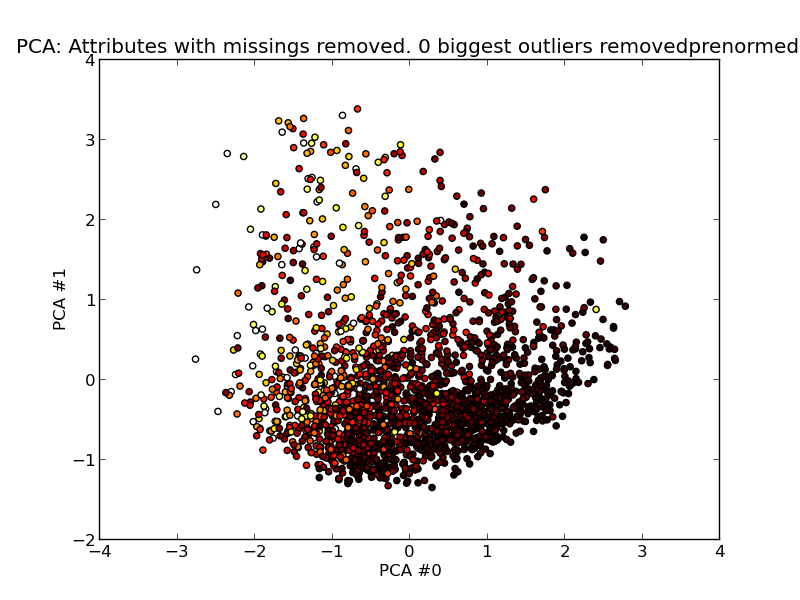
\includegraphics[width=\textwidth]{pca/attr-with-missings-removed_0-biggest-outliers-removed_prenormed_}
\end{figure}
\end{minipage}
\hfill
\begin{minipage}{0.4\textwidth}
\begin{figure}
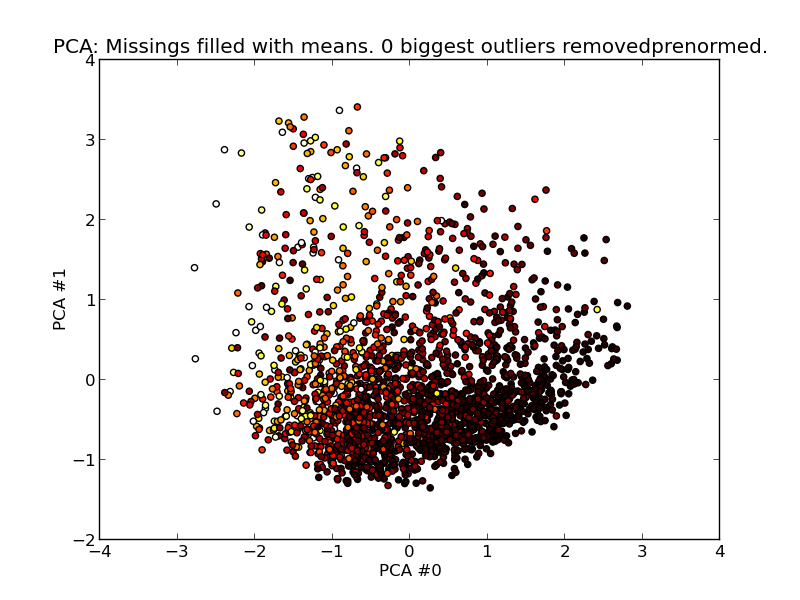
\includegraphics[width=\textwidth]{pca/missings-filled-w-means_0-biggest-outliers-removed_prenormed_}
\end{figure}
\end{minipage}
[PCA WITH PRENORMED DATA]

The above data also appears to be normally distributed, in contrast to our own PCA.

[bad correlation]

Most of out attributes have little correlation, as seen above, which is why regression is an obvious machine learning task. Looking at the normalized data by [WHO], furthermore leads us to believe that the task is feasable.
